\chapter{需求分析}
需求分析是软件工程生命周期中十分关键的环节，其主要任务是通过对用户需求、业务场景和实际问题的梳理，将较为抽象的业务想法转化为清晰、可执行、可验证的需求说明。需求分析的质量直接影响系统建设的范围、设计方向以及最终交付效果，是连接业务目标与技术实现的重要基础。

本章围绕企业数字化运营平台的建设需求展开分析。首先，对系统应具备的总体功能进行概述，使读者能够从整体上了解系统建设的背景和意义；随后，进一步从功能需求和非功能性需求两个方面进行分析。其中，功能需求主要描述系统各业务模块应实现的具体功能，是后续系统架构设计、模块划分和业务流程设计的重要依据。非功能性需求则主要关注系统在实际运行过程中的稳定性、安全性、可扩展性和易用性等方面，既要保证系统能够长期稳定运行，也要提升用户在使用过程中的流畅性、便捷性和可靠性。

\section{系统总体需求概述}
本系统是某汽车电子公司内部的数字化运营管理系统，面向企业内部的软件项目管理和运营管理场景，主要用于解决项目过程数据分散、统计分析依赖人工整理、业务流程跟踪不能自动化等问题。系统需要将项目、组织、人员、工时、质量和运营指标等数据进行整合，为管理人员提供较为统一的数据查看和业务处理平台。

从业务范围上看，系统主要包括三个部分。第一部分是项目管理，围绕项目基础信息、版本范围、质量问题和风险事项等内容，对项目执行过程进行记录、查询和跟踪。第二部分是公司运营管理，主要面向组织、员工、工时和 KPI 等运营数据，支持从部门、人员、项目等角度进行统计分析。第三部分是系统管理，该部分主要作为系统基础支撑，提供用户、角色、菜单、部门、权限和日志等后台管理功能，为业务模块的正常运行提供支撑。
\begin{figure}[htbp]
	\centering
	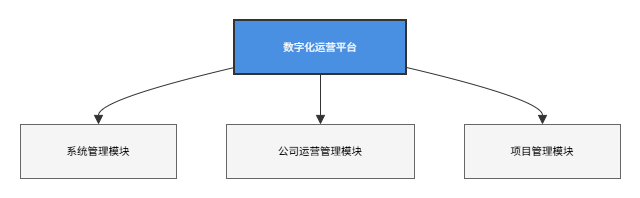
\includegraphics[width=0.68\linewidth]{imgs/总体模块图.png}
	\caption{玄武平台模块图}
	\label{fig:xuanwu-module}
\end{figure}

系统的使用对象包括项目经理、部门经理、项目成员（开发测试人员）以及质量管理人员等。不同角色在系统中的关注内容和操作权限不同，因此系统需要具备统一的身份认证、权限控制和数据访问管理能力，以保证业务数据的安全性。本系统的建设目标是将项目管理、运营分析和系统基础管理整合到同一平台中，减少分散系统和人工统计带来的管理成本，提高企业内部项目过程管理和运营数据分析的效率。

\section{功能需求}
在系统总体需求的基础上，本节结合毕业设计任务分工，对本文负责实现的功能模块进行需求分析。本文的实现范围主要包括公司运营管理模块中的部门投入 BU 工时统计功能，以及项目管理模块中的项目基础信息管理、缺陷管理和重大问题管理功能。上述功能分别对应运营数据分析和项目过程管理两个方面，是系统整体业务中的一部分。

在相关功能中，部门经理主要关注部门工时在不同 BU 方向上的投入情况；项目经理主要负责项目基础信息维护和项目过程跟踪；项目成员（开发测试人员）参与缺陷和重大问题的处理与反馈；质量管理人员则重点关注缺陷数据、重大问题状态以及相关质量风险。为便于后续系统设计，下面将按照功能模块分别分析各功能的参与角色、业务目标和主要操作需求。

\subsection{部门投入BU工时统计需求分析}
BU工时投入分析模块旨在为部门经理提供下属员工在各BU（Business Unit）上工时分布的全景视图，为人力资源调配与项目成本核算提供数据支撑。该模块仅涉及部门经理一类参与者。如图\ref{fig:bu-usecase}所示，系统需要提供按年月和组织树两个维度的工时数据检索能力，支持以饼图形式呈现部门整体的BU工时分布情况。同时，系统需要支持对特定BU的工时数据进行详细分析，提供总工时、平均工时和加班工时等基础统计指标的计算能力，并能够生成近六个月的工时趋势图，以便识别工时投入的变化规律。
\begin{figure}[htbp]
	\centering
	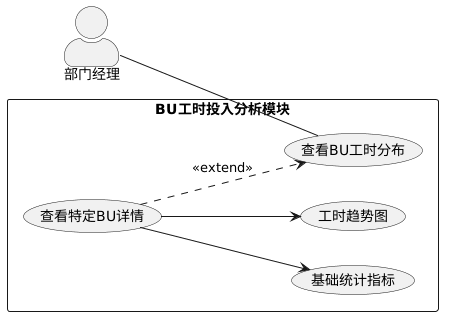
\includegraphics[width=0.68\linewidth]{imgs/usecase/部门投⼊到BU的⼯时分布用例图.png}
	\caption{BU工时分布用例图}
	\label{fig:bu-usecase}
\end{figure}

\subsection{项目信息管理需求分析}
项目信息管理模块需要支持项目经理、项目成员这两类参与者对项目基本信息和里程碑计划的。如图\ref{fig:project-usecase}所示，该模块可划分为项目基本信息和里程碑计划两个子域。在项目基本信息方面，系统需要支持项目信息的新增、编辑、查询和导出能力，其中项目经理拥有完整的写权限，部门经理和普通用户仅具备只读权限。在里程碑计划方面，系统需要支持项目周报的填写、修改和查询，以及交付历史的查看，确保各角色能够在各自权限范围内获取所需的项目进度信息。
\begin{figure}[htbp]
	\centering
	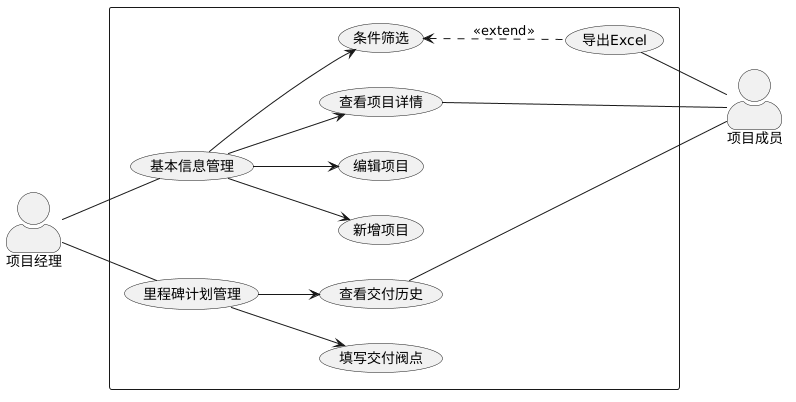
\includegraphics[width=0.68\linewidth]{imgs/usecase/项目信息管理用例图.png}
	\caption{项目信息管理用例图}
	\label{fig:project-usecase}
\end{figure}


\subsection{缺陷管理需求分析}
缺陷管理模块需要解决企业内部缺陷数据分散在多个异构平台中的问题，实现缺陷信息的统一归集与聚类分析。如图\ref{fig:defect-usecase}所示，该模块的用例可归纳为缺陷查看与项目聚类管理两大部分。在缺陷查看方面，系统需要对接Trinity、Jira和BugClose三个外部缺陷跟踪平台，将分散的缺陷数据统一汇总，并支持按项目、集群、时间等多维度进行条件筛选和详情查看，三类角色均可使用该能力。在项目聚类管理方面，系统需要支持项目聚类的增删改查操作，并提供聚类下项目列表和缺陷详单的查看能力；当缺陷数量达到预警阈值时，系统需要具备通过飞书向相关人员发送预警消息的能力。此外，系统还需要支持缺陷数据的Excel导出，便于线下分析和汇报。
\begin{figure}[htbp]
	\centering
	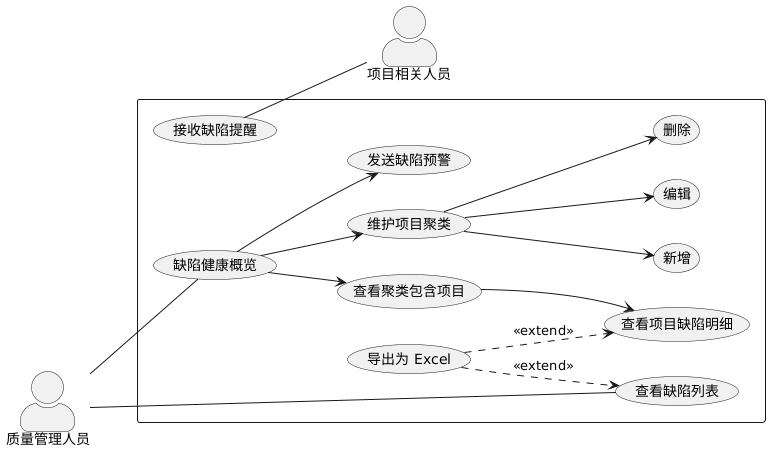
\includegraphics[width=0.68\linewidth]{imgs/usecase/缺陷管理用例图.png}
	\caption{缺陷管理用例图}
	\label{fig:defect-usecase}
\end{figure}

\subsection{重大问题管理需求分析}
重大问题管理模块需要对项目中出现的高影响风险问题提供从登记、跟踪到闭环处置的全流程管理能力。如图\ref{fig:critical-usecase}所示，系统需要支持重大问题的新建、编辑、查询和导出功能，其中编辑功能需要涵盖根因分析、关闭信息填写和问题上升标记三种处置动作。在通知机制方面，系统需要在问题新建或上升时具备通过飞书卡片消息向管理层推送通知的能力。在监督层面，系统需要支持重大问题列表查看、统计图表展示和数据导出，并支持在需要时主动触发飞书催办。此外，当重大问题需要横向扩散时，系统需要支持在问题关闭阶段将横展信息同步推送到其他可能存在相同风险的项目中，确保问题不被遗漏。该模块涉及部门经理、项目经理和普通用户三类参与者，如图\ref{fig:critical-usecase}所示。
\begin{figure}[htbp]
	\centering
	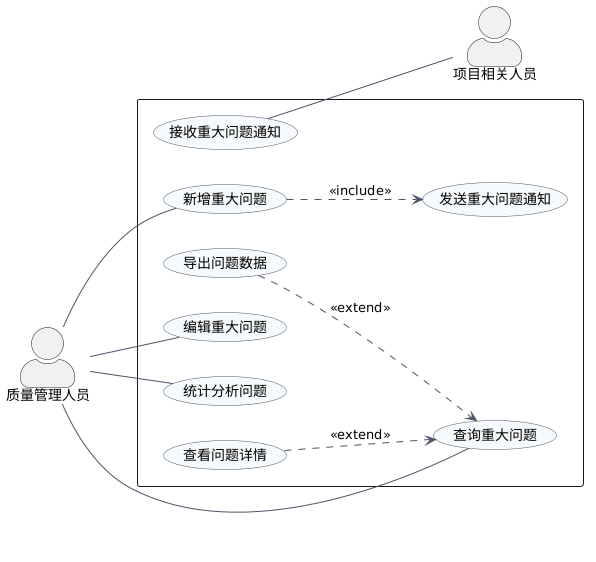
\includegraphics[width=0.68\linewidth]{imgs/usecase/重大问题用例图.png}
	\caption{重大问题用例图}
	\label{fig:critical-usecase}
\end{figure}

\section{非功能需求}
前文主要对系统的核心业务用例和功能流转进行了梳理。但在实际的企业生产环境中，除了要满足基础的业务逻辑外，系统还必须具备在长周期运营与高频使用中的可用性与可靠性，因此，在实际编码之前，本平台还需要满足以下几个关键的非功能性指标。

\subsection{性能要求}
按照汽车软件研发团队的规模推算，系统上线后，底层的工时流水记录和历史缺陷明细表的数据量会在短时间内快速增长，导致单张数据表的体积非常大。这就要求系统在处理涉及多表关联和分组聚合统计时，不能出现严重的慢查询。特别是对于前端首页通过 ECharts 渲染的 BU 工时看板和项目健康度图表，规定相关数据接口的响应时间必须控制在用户可接受的范围以内。如果因为底层数据量过大导致页面出现长达几秒的“白屏”，或者直接抛出请求超时异常，是实际业务无法接受的，因为这非常影响用户的体验。

\subsection{外部接口的容错性}
由于该项目的后端设有定时任务，需要定时调用外部的飞书 API 来向满足条件的用户发送飞书卡片进行催办。但在真实网络环境下，第三方接口随时都可能出现限流、网络波动或定时任务运行出错。因此，系统设计时必须考虑相应的容错处理。具体来说，当调用飞书接口超时或失败时，当前任务线程不能直接崩溃，同时，涉及业务变更的数据库操作必须触发事务回滚，防止产生脏数据。此外，系统需要把这类外部调用异常的堆栈信息完整地输出到日志文件中，并在连续失败时主动向管理员发送告警，以便人工介入排查。

\subsection{接口的健壮性}
Web 应用开发的一个基本原则是“永远不要相信前端传来的数据”。为了防止非法参数引发后台的空指针异常或越权漏洞，所有 Controller 层的入口都必须接入严格的参数校验逻辑，把无效请求直接挡在业务代码之外，降低系统不必要的运算消耗。另一方面，考虑到高并发场景，一些恶意查询或者异常前端代码会频繁查询数据库中不存在的数据，就会导致 Redis 缓存永远无法命中，所有的请求都越过缓存这道防线到达底层数据库，极易引发数据库连接池耗尽甚至宕机。因此，需要采取具体的策略来进行防范，比如最简单的操作就是缓存一些空对象，并设置合适的过期时间。

\subsection{易用性}
由于该运营平台的使用者涵盖了从普通外包测试员工到高层 PMO 经理，各自的使用习惯差异很大，这就要求前端界面不能设计得过于繁琐。前端界面需采用现代化的扁平化设计与组件化交互规范，降低操作门槛。特别是在处理含有几十个字段的工时填报表单或缺陷长列表时，必须做好数据的异步加载、分页以及按钮的“防抖”处理（防止用户手抖连续点击提交）。当数据保存成功或后台校验失败时，系统必须通过全局的消息组件给出明确的中文提示，避免给用户造成“点不动”或“系统卡死”的错觉。

\section{本章小结}
本章围绕企业数字化运营平台的建设目标，从总体需求、功能性需求和非功能性需求三个层面，对系统进行了全面梳理与深度分析。首先从普通员工、项目经理、部门经理等核心用户的视角出发，分析出他们各自的需求。在此基础上，将待实现的功能需求按照业务领域重新聚合，同时从性能、容错、安全与易用性等角度提出了系统在高并发、大数据量场景下的非功能约束。下一章将基于此需求规格，通过描述系统的概要设计来阐述系统的整体架构设计。

